%**************************************************************
% Capitolo 1 - L'azienda
%**************************************************************
\chapter{L'azienda\label{cap:lazienda}}
\begin{figure}[H]
   \begin{center}
      
\includegraphics[width=10cm,height=1.5cm,keepaspectratio]{immagini/vla-logo}
   \end{center}
   \caption{Logo di \nomeAziendaComm{}}\label{logovla}
\end{figure}
\nomeAziendaComm{} è una startup nata a New York nel 2011, con sede operativa a Torri di Quartesolo (VI), impegnata nello sviluppo di tecnologie di \engl{\gls{ubiquitous computing}} per i settori sanitario, manifatturiero e della sicurezza.

\section{Prodotti e servizi}
I prodotti principali di \nomeAzienda{} sono software personalizzati, siti web e contenuti video. L'azienda, inoltre, offre un servizio pubblicitario per le nuove aziende: costruisce il \engl{{brand}} del cliente, pone le fondamenta della sua rete di clienti e si occupa di consulenze e di \engl{\gls{SEO}}.
\\
Con il crescere del team e l'acquisizione di nuovo personale più specializzato, \nomeAzienda{} si sta espandendo verso servizi cloud per le aziende e software per dispositivi \engl{\gls{wearable}} e \engl{\gls{IoT}}; questi sono i primi approcci al modello di \engl{\gls{ubiquitous computing}} e permettono ai loro utenti una maggiore integrazione con la rete di informazioni e sensori che li circondano nella vita quotidiana. L'azienda sta sviluppando particolarmente il campo dei visori per realtà aumentata come supporto alle attività lavorative, promettendo grandi innovazioni nel settore manifatturiero.

\section{Come lavora}

   \subsection{Modello di sviluppo}
   \nomeAzienda{} lavora con il modello di sviluppo \engl{Agile} di tipo \engl{Scrum}. Questo modello pone una minore rigidità sulla documentazione e sulle formalità del prodotto, permettendo modifiche in corso d'opera e una collaborazione più rilassata tra cliente e fornitore.

   \begin{figure}[htbp]
      \centering
      \includegraphics[width=14cm]{immagini/scrum-process}
      \caption[Ciclo di vita di Scrum]{Ciclo di vita di Scrum
      \\
      Source: Wikimedia Commons, Lakeworks, CC}
   \end{figure}
   %TODO: creare un'immagine migliore

   \engl{Scrum} definisce uno \engl{sprint} come l'unità di misura dello sviluppo di un progetto, un periodo di tempo di lunghezza fissata generalmente tra una settimana e quattro settimane.
   L'insieme delle attività necessarie per l'avanzamento del progetto sono organizzate nel \engl{backlog} del prodotto.
   Per ogni \engl{sprint} il team pianifica quali di questi \engl{task} dovranno essere svolti e a chi andrà assegnato ciascuno di essi, definendo così il \engl{backlog} dello sprint.
   \\
   Ogni giorno il team si ritrova con una breve riunione, detta ``\engl{daily scrum}'', per controllare lo stato dei \engl{task} e degli obiettivi. I \engl{meeting} giornalieri permettono al \gls{project manager} di avere misure dello stato del progetto con più frequenza, rispetto a altri modelli di sviluppo, così da intervenire più rapidamente alla necessità di correzioni.
   \\
   Un vantaggio del modello \engl{Scrum}, e in generale dei modelli agili, è quello di poter vedere il risultato del proprio lavoro più in fretta rispetto ai metodi tradizionali: i \engl{daily scrum} servono anche a incentivare gli sviluppatori e a fornire loro una sensazione di progresso, che, invece, viene persa se i tempi tra un aggiornamento e l'altro si dilatano.
   \\
   Un ulteriore punto di forza di \engl{Scrum} è il legame di cooperazione che si forma tra il fornitore e il cliente: questo si sente parte del team ed è più propenso a offrire e a ricevere opinioni costruttive, con minori impuntamenti e risultati migliori per entrambe le parti.
   \\
   Trattandosi di un modello \engl{Agile} la documentazione è molto più ridotta rispetto ai metodi tradizionali: nasce il concetto di user story, un documento che descrive le richieste del cliente e le decisioni prese assieme a quest'ultimo sul progetto durante incontro faccia a faccia. Il vantaggio principale di questo tipo di documentazione è la snellezza dei documenti, sia quando devono essere consultati, sia quando devono essere scritti. Avere una visione chiara di ciò che il cliente vuole può essere difficile se è necessario scorrere decine di pagine di verbali per ottenere tali informazioni; così, al contrario, è sufficiente controllare le ultime decisioni prese.
   \\
   Il coordinamento del lavoro viene gestito tramite fogli di calcolo con funzioni automatiche, condivisi all'interno del team. Per ogni \engl{task} è segnalato il livello di avanzamento, che deve essere aggiornato da colui a cui è stato assegnato, riportando il tempo impiegato ed eventuali note.
   \\
   Gli stati in cui un \engl{task} si può trovare sono i seguenti:
   \begin{itemize}
      \item{\textbf{Analysis}: il \engl{task} richiede analisi}
      \item{\textbf{Pending}: il \engl{task} è definito ed è in attesa di essere svolto}
      \item{\textbf{Blocked}: il \engl{task} è bloccato a causa delle sue dipendenze}
      \item{\textbf{Development}: il \engl{task} è in svolgimento}
      \item{\textbf{Testing}: il prodotto è in fase di test}
      \item{\textbf{Reworking}: lo sviluppo è fallito e sta venendo rieseguito}
      \item{\textbf{Refactoring}: il codice prodotto è in fase di pulizia}
      \item{\textbf{Completed}: lo sviluppo è completato}
      \item{\textbf{Confirmed}: il \engl{task} è stato validato}
   \end{itemize}
   Il sistema di tracking del tempo impegnato da ciascun \engl{task} aiuta il project manager a valutare lo stato del progetto, confrontandolo con le stime fatte a preventivo.

   \subsection{Progetti importanti}
   \subsubsection{VisionHealthCare}
   VisionHealthCare è un software prodotto da \nomeAzienda{} in collaborazione con Dedalus Spa\footnote{Sito web di Dedalus Spa: \href{http://www.dedalus.eu}{www.dedalus.eu}}, società leader nazionale nel software clinico sanitario. L'applicazione, legata a OrmaWeb, suite applicativa web di Dedalus Spa, sfrutta gli occhiali per la realtà aumentata di Google, i Google Glass, per automatizzare e semplificare ogni fase del percorso chirurgico, dalla lista d'attesa alla gestione del blocco operatorio, fino alla produzione del registro operatorio e la redazione della cartella anestesiologica pre e intraoperatoria.
   \begin{figure}[H]
      \begin{center}
         
\includegraphics[width=15cm,keepaspectratio]{immagini/visionhealthcare-schema}
      \end{center}
      \caption{Schema di funzionamento di VisionHealthCare}\label{schemavisionhealthcare}
   \end{figure}
   I Google Glass si interfacciano con un'applicazione installata in uno smartphone e si collegano tramite questo ai servizi di OrmaWeb.
   Gli occhiali permettono di registrare note vocali correlate da video e foto, utili alla documentazione dell'operazione. Il sistema permette di automatizzare buona parte delle procedure di verbalizzazione dell'intervento, trascrivendo il testo registrato e aggiungendolo ai dati salvati su OrmaWeb. Un ulteriore utilizzo dei dati registrati è quello educativo: spesso l'unica persona in sala operatoria ad avere un buon punto di vista sull'operazione è il chirurgo che la sta praticando, ma questo non ha la possibilità di reggere una videocamera. Una soluzione di questo tipo permette di lavorare con le mani libere e allo stesso tempo di ricevere dati aggiuntivi sullo stato del paziente, come il suo battito cardiaco o la quantità di ossigeno nel sangue.

   \subsubsection{NapkinForever --- Paperworld 2017}
   \nomeAzienda{} sta collaborando con NapkinForever\footnote{Sito web di NapkinForever: \href{www.napkinforever.com}{www.napkinforever.com}}, azienda italiana di penne e stilo di design, per realizzare una presentazione virtuale dell'impresa per il Paperworld 2017, la più grande fiera al mondo di prodotti per gli uffici e strumenti di scrittura. Il progetto consiste in una simulazione realizzata tramite l'utilizzo dei Google Cardboard, gli occhiali per la realtà virtuale di Google, che accompagnerà i visitatori nel mondo del design di NapkinForever e presenterà loro i prodotti dell'azienda.
   \begin{figure}[H]
      \begin{center}
         \includegraphics[width=15cm,height=5cm,keepaspectratio]{immagini/cardboard-schema}
      \end{center}
      \caption{Schema di funzionamento di Google Cardboard}\label{schemacardboard}
   \end{figure}
   I Google Cardboard consistono in un apparato di lenti, da applicare allo schermo di uno smartphone, e di un telaio in cartone. L'utilizzo di hardware comune e di materiali poveri permette di mantenere il prezzo del dispositivo molto basso rispetto ai competitor, pur fornendo una buona esperienza d'uso. La simulazione permetterà di visualizzare i prodotti proposti dall'azienda in scenografie ad hoc e di ottenere informazioni contestuali su di essi.

   \subsection{Premi e certificazioni}

   \subsubsection{Unicredit Start Lab}
   \begin{figure}[H]
      \begin{center}
         \includegraphics[width=6cm,height=3cm,keepaspectratio]{immagini/unicreditstartlab-logo}
      \end{center}
      \caption{Logo di Unicredit Start Lab}\label{logounicreditstartlab}
   \end{figure}
   \nomeAzienda{} ha partecipato alla competizione tra startup Unicredit Start Lab\footnote{Sito web Unicredit Start Lab: \href{http://www.unicreditstartlab.eu}{www.unicreditstartlab.eu}} 2017, durante la quale le aziende partecipanti hanno proposto i propri progetti innovativi nei campi ``Digital'', ``Clean Tech'' e ``Innovative Made in Italy''. L'azienda si è classificata tra i 10 finalisti e ottenendo un periodo di incubazione e accelerazione da parte di Unicredit a partire da Settembre 2017.

\section{Tecnologie utilizzate dall'azienda}
%TODO: rimuovere i loghi e aggiungere informazionis sull'architettura interna, esterna e di uso
%TODO: commentare le illustrazioni
L'azienda fa uso di un gran numero di tecnologie durante le proprie attività; di seguito analizzerò le più utilizzate.

   \subsection{Rackspace}
   Rackspace è un cloud provider che offre servizi di managed cloud computing, basati su \gls{VPS} e altri servizi cloud, come \gls{AWS}, Microsoft Azure e OpenStack. Questo tipo di servizio permette di gestire facilmente servizi cloud utilizzati, mantenendo il pieno controllo di costi e infrastrutture, senza la necessità di conoscere a fondo ogni componente utilizzato.
   \begin{figure}[H]
      \begin{center}
      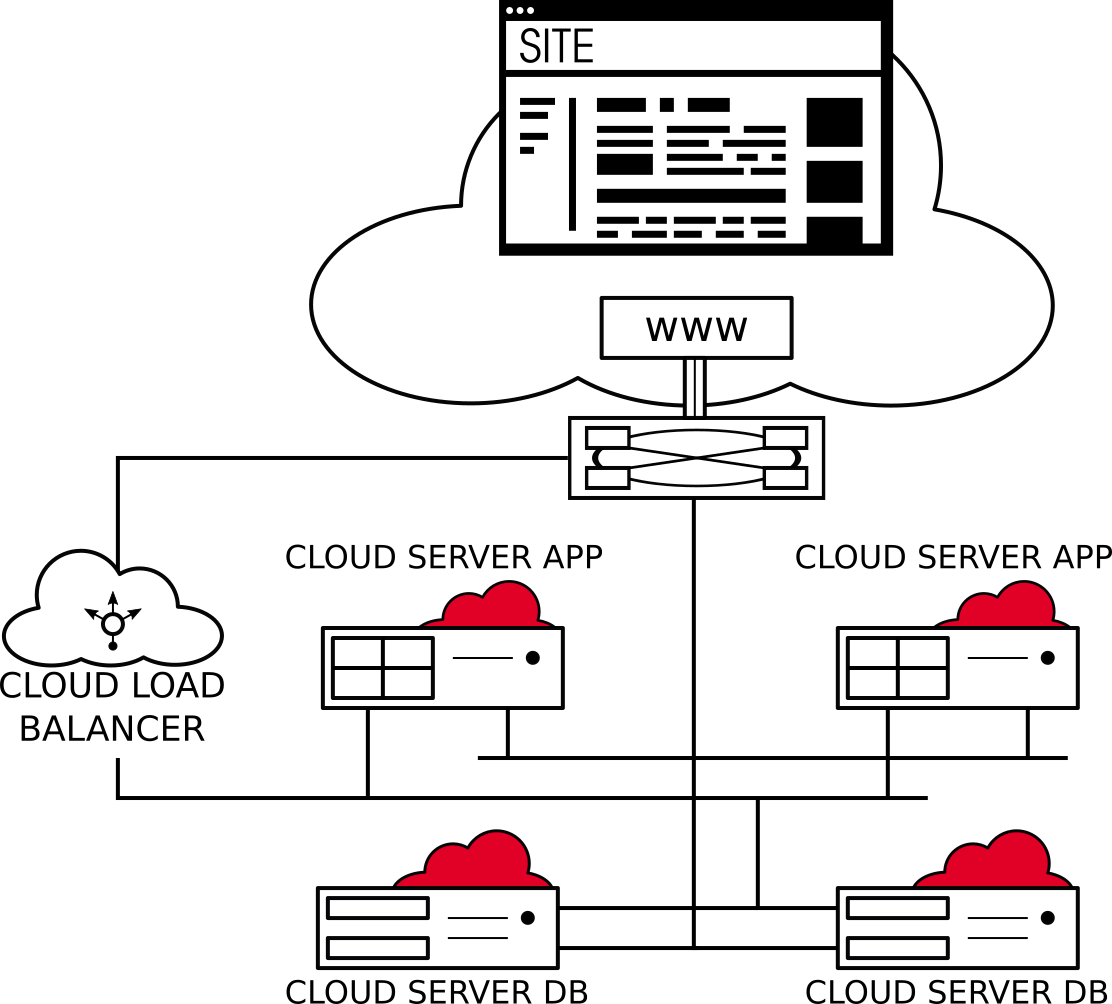
\includegraphics[width=14cm,keepaspectratio]{immagini/rackspace-network}
      \end{center}
      \caption{Schema di rete generale di un'applicazione su Rackspace}
   \end{figure}
   Rackspace permette di gestire in modo semplice nodi per il load balancing e la ridondanza dei servizi. In questo modo è possibile garantire up-time estremamente elevati e distribuire gli aggiornamenti sui singoli nodi, senza mai fermare il servizio completamente.
   \\
   \nomeAzienda{} usa Rackspace come hosting provider nel caso di progetti complessi, quando è necessaria una completa gestione delle risorse.

   \subsection{Firebase}
   Firebase è una piattaforma di sviluppo per applicazioni Web e mobile, parte di Google Cloud Platform; fornisce servizi di scambio di messaggi e basi di dati in tempo reale, spazio di archiviazione, sistemi di autenticazione, web hosting e test automatici per applicazioni Android. La piattaforma fornisce anche un servizio di analisi e profilazione degli utenti e l'integrazione con il sistema di annunci pubblicitari di Google, AdMob.
   \begin{figure}[H]
      \begin{center}
         \includegraphics[width=14cm,keepaspectratio]{immagini/firebase-usecase}
      \end{center}
      \caption{Usecase generale di Firebase}
   \end{figure}
   Il caso d'uso principale di Firebase è quello di base di dati per la sincronizzazione di dati tra dispositivi, anche su piattaforme diverse, in tempi molto ridotti. A differenza di un database non relazionale comune, il servizio che Firebase offre si basa su una CDN molto estesa, che permette di ridurre i tempi di attesa per la sincronizzazione dei dati.
   \\
   \nomeAzienda{} utilizza Firebase quando necessita della creazione di un ambiente di sviluppo completo, veloce e facile da manutenere.

   \subsection{Java}
   Java è un linguaggio di programmazione ad alto livello orientato agli oggetti pensato per essere il più possibile indipendente dalla piattaforma sulla quale viene eseguito. Java supera questo ostacolo utilizzano una macchina virtuale, la JVM, che permette di astrarre il sistema sottostante. Il vantaggio di Java sui linguaggi compilati tradizionali è proprio quello di poter essere eseguito su una qualsiasi piattaforma, a patto che esista una JVM per questa.
   \begin{figure}[H]
      \begin{center}
         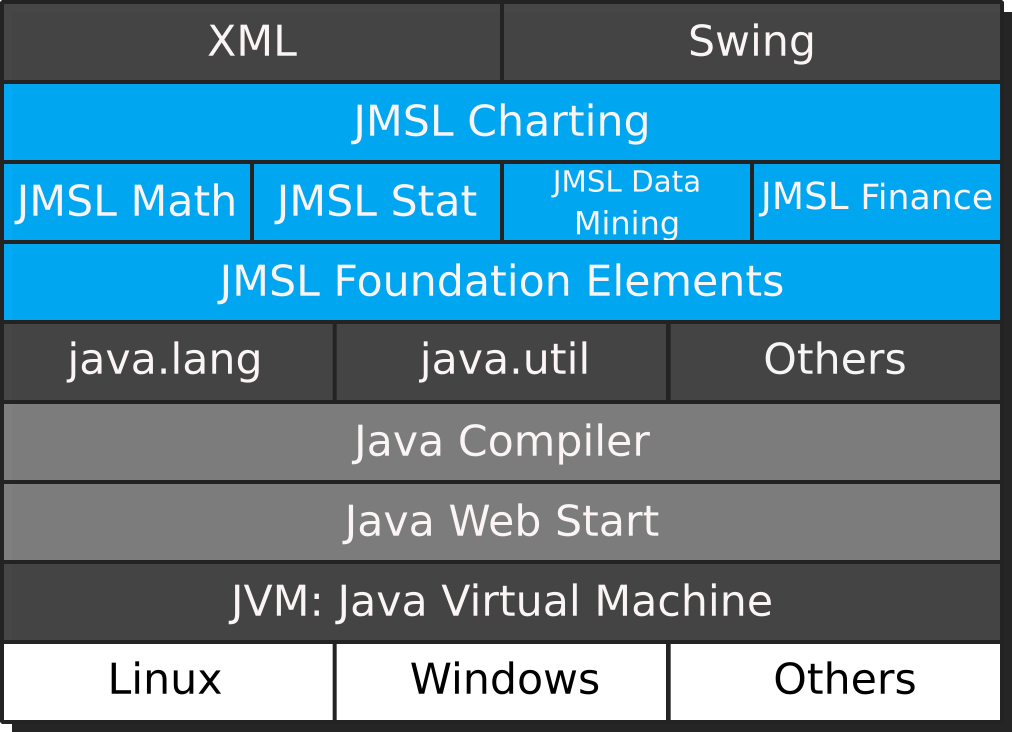
\includegraphics[height=7cm,keepaspectratio]{immagini/java-architecture}
      \end{center}
      \caption{Architettura di Java}
   \end{figure}
   Tra le tecnologie utilizzate da \nomeAzienda{} troviamo Android, fortemente basato su Java, e utilizzato per la creazione di applicazioni per dispositivi mobile. Molti dei progetti passati dell'azienda sono legati ad applicazioni Android, ma \nomeAzienda{} utilizza Java anche nel caso di servizi web ad alto parallelismo.
   \begin{figure}[H]
      \begin{center}
         \includegraphics[width=14cm,height=18cm,keepaspectratio]{immagini/android-stack}
      \end{center}
      \caption[Architettura di Android]{Architettura di Android
      \\
      Source: \href{https://developer.android.com/guide/platform/index.html}{Documentazione Android Developers}}
   \end{figure}
   Android consiste di una versione minimale del kernel Linux, completo di driver specializzati per l'hardware del dispositivo sul quale verrà installato. Al di sopra del kernel si trova un layer di astrazione dell'hardware. Questo layer permette agli strati superiori di astrarre l'hardware sottostante. Il layer superiore contiene librerie native in C o C++, altamente efficienti, e il runtime Android, l'equivalente della JVM in Java, ma specializzato per l'esecuzione su dispositivi mobile e fortemente integrato con le librerie e l'hardware sottostante. Gli strati superiori sono, infine un'API per l'accesso alle risorse del sistema e le applicazioni. Queste sono racchiuse in contenitori e le autorizzazioni di queste possono essere gestite singolarmente.

   \subsection{Git e Bitbucket}
   \nomeAzienda{} utilizza Git come \gls{CVS} per il versionamento del codice: Git è in grado di gestire progetti anche molto complessi in modo efficiente. Il suo sistema completamente distribuito permette a due persone di lavorare contemporaneamente sullo stesso file, senza necessità di una connessione di rete, e di conservare copie sicure del prodotto in luoghi separati, pur garantendone la consistenza.
   \begin{figure}[H]
      \begin{center}
         
\includegraphics[width=15cm,height=3cm,keepaspectratio]{immagini/git-branches}
      \end{center}
      \caption[Esempio di grafo di lavoro in Git]{Esempio di grafo di lavoro in Git
      \\
      Source: Wikimedia Commons, Bunyk, CC}\label{grafogit}
   \end{figure}
   Nell'esempio in Fig.~\ref{grafogit} due sviluppatori hanno lavorato in parallelo in un repository Git, ciascuno in un branch separato, dando origine ad alcuni commit (i nodi A, B, C, D e W, X, Y, Z). Successivamente è stato eseguito un merge, un unione tra i due branch, che ha generato il nodo Z'. Nel caso di conflitti tra le righe di codice scritte o modificate, Git è in grado di valutare quali sono i \engl{chunk} di codice da controllare e lascerà agli sviluppatori il compito di risolverli.
   \\
   Per facilitare la gestione del codice e automatizzare alcune attività, l'azienda ha scelto di utilizzare Bitbucket come hoster per le proprie repository. Bitbucket integra il servizio di pipeline, che permette di eseguire degli script in ambienti virtualizzati basati su Docker; in questo modo sono stati automatizzati i test di unità e integrazione e i controlli della quality assurance. Questo tipo di operazioni fanno risparmiare tempo, dato che non necessitano dell'intervento umano, inoltre la garanzia che ogni commit al repository è stato testato conferisce la sicurezza di poter rilasciare una nuova versione senza riserbo.
   \begin{figure}[H]
      \begin{center}
         \includegraphics[width=15cm,height=6cm,keepaspectratio]{immagini/bitbucket-pipeline}
      \end{center}
      \caption{Schema generale di una pipeline in Bitbucket}\label{pipelinebitbucket}
   \end{figure}
   La configurazione tipica di una pipeline su Bitbucket segue il seguente iter:
   \begin{enumerate}
      \item{Uno sviluppatore carica sul server Bitbucket del codice, tramite un push di Git;}
      \item{Il server Bitbucket carica il codice in un contenitore Docker, secondo la configurazione del repository;}
      \item{Il contenitore esegue la configurazione dell'applicazione e lancia tutti i test, restituendone i risultati al server;}
      \item{Se i test vengono superati il commit viene ritenuto valido, altrimenti può essere scartato;}
      \item{Se il codice è stato caricato su un ramo di release, il nuovo commit viene caricato su un nuovo contenitore Docker, che si occuperà della creazione di una build del prodotto;}
      \item{Lo stesso Docker può essere configurato in modo tale da caricare il prodotto compilato sui server di produzione, oppure avvisare un certo gruppo di persone di eseguire ulteriori test sulla build ottenuta.}
   \end{enumerate}
   In caso di fallimento di uno dei task della pipeline, lo sviluppatore che ha caricato il codice viene avvisato degli errori e gli vengono forniti i log delle operazioni eseguite.


   \subsection{G Suite}
   G Suite, la soluzione per l'ufficio di Google, offre una gestione completa di mail commerciali, editor di testo, fogli di calcolo, calendario e archivio di dati; il tutto tramite una semplice interfaccia web.
   \begin{figure}[H]
      \begin{center}
      \includegraphics[width=16cm,keepaspectratio]{immagini/g-suite-products}
      \end{center}
      \caption{I prodotti di G Suite}
   \end{figure}
   Tra i prodotti più utilizzati di G Suite si notano Drive, il servizio di storage; Docs, Spreadsheet e Slides, rispettivamente per documenti di testo, fogli di calcolo e presentazioni; Gmail, per la gestione delle mail aziendali. G Suite include anche un servizio per la gestione di contatti, calendari e un servizio di video chat.
   \\
   \nomeAzienda{} usa questo servizio per le proprie attività, soprattutto per il vantaggio di poter accedere ai dati salvati anche in mobilità, con la massima comodità.

   \subsection{WordPress}
   WordPress è \gls{CMS} open-source che offre una piattaforma editoriale personale; nato per gestire semplici blog, viene utilizzato come framework di sviluppo di siti molto più complessi, sfruttando il sistema a plugin su cui e basato. L'utilizzo di WordPress come base di un sito permette di iniziare a lavorare con un framework riutilizzabile, stabile e aggiornato che ne gestisce i contenuti e i dati, permettendo allo sviluppatore di concentrarsi sulla loro presentazione all'utente.
   \begin{figure}[H]
      \begin{center}
         \includegraphics[width=16.5cm,keepaspectratio]{immagini/template-hierarchy}
         \caption[Architettura di una pagina WordPress e gerarchia delle pagine]{Architettura di una pagina WordPress e gerarchia delle pagine
         \\
         Source: \href{https://developer.wordpress.org/themes/basics/template-hierarchy/}{WordPress Developer Documentation}}
      \end{center}
   \end{figure}
   WordPress organizza i contenuti come pagine o articoli; predispone un archivio per organizzarli e un sistema di ricerca basato sui testi e sui metadati legati. La home del sito ha il compito di mostrare i contenuti più recenti o più importanti del sito e permette di scorrere tutti gli articoli come una vetrina.
   \\
   \nomeAzienda{} sfrutta WordPress come base dei propri siti anche per rendere la modifica dei contenuti semplice al proprio cliente.

\section{Rapporto con l'innovazione}
\nomeAzienda{} è da sempre alla continua ricerca di nuove tecnologie da conoscere e integrare nei propri prodotti, anche in campi sperimentali, come i dispositivi \gls{wearable}, \gls{IoT} e la realtà aumentata. Proprio questi ultimi hanno dato origine ad alcuni dei progetti più all'avanguardia dell'azienda e l'hanno spinta all'acquisizione di personale dedito alla sperimentazione di nuove soluzioni.
\\
Un'ulteriore necessità di innovazione deriva dal settore nel quale \nomeAzienda{} si propone: il mercato è in rapida crescita e questo impone un continuo aggiornamento delle conoscenze e delle tecniche per mantenere i propri prodotti validi e restare al passo con i competitor.
\\
Testimonianza di questo continuo aggiornamento è la migrazione verso uno sviluppo cloud based di molti dei prodotti dell'azienda, che ha portato a una riduzione dei costi di manutenzione e a un maggiore controllo sulla disponibilità dei servizi.
\\
L'azienda, inoltre, organizza seminari periodici e laboratori per informare ed aggiornare i propri componenti sulle ultime frontiere della tecnologia, in ambito di sviluppo e marketing.
\\
La proposta di nuove tecnologie è libera all'interno dell'azienda e, se ritenute utili per progetti futuri, viene predisposto un piccolo progetto di prova. In questo modo si riescono a ottenere dati concreti sui vantaggi e gli svantaggi che possono offrire.
